%!TEX root = ../username.tex
\chapter[J.S. Bach and \textit{The Well-Tempered Clavier} BWV 847]{Johann Sebastian Bach – \textit{The Well-Tempered Clavier Prelude and Fugue in C Minor}, BWV 847 (1722 and 1740)}\label{bach}

Johann Sebastian (J.S.) Bach (1685-1750) is a composer of the Baroque period, which is commonly approximated to be from about 1600 to 1750. He was born on March 31, 1685, in Leipzig, Germany, and is celebrated as the creator of influential works that include \textit{The Well-Tempered Clavier}, \textit{St. Matthew's Passion}, and \textit{Mass in B Minor}. His works are identified by their number in Wolfgang Schmeider's catalog, as Bach-Werke-Verzeichnis (BWV, or in English, "Bach's work catalog"). This catalog was first published in 1950, and groups compositions by genre. Das wohltemperierte Clavier (published as two books, the first in 1722 and the second in 1740) is one of Bach's best-known keyboard works. It is translated to English as \textit{The Well-Tempered Clavier}, and is commonly referred to as WTC \autocite{Lindley_2001}.

The two books in WTC consist of 24 prelude and fugue pairs, in alternative major and minor keys. The pairs start in C Major, and are arranged in a rising chromatic pattern, ending in B Minor. The first prelude and fugue pair is in C Major, the second pair is in C Minor, the third in D Major, and so on until the last pair reaches B Minor. WTC was composed to demonstrate the possibilities of playing in every key in an equal-, or near-equal temperament, which was a new concept. 

Temperament is the name given to various tuning methods, in which consonant intervals, mainly the third and the fifth interval, are made to be more or less imperfect, which is to say they are made to be sharper or flatter than they are originally intended \autocite{Grove_1895}. The phrase \say{well-tempered} refers to the use of a tuning system which works equally well in all keys. An octave is divided into 12 semitones of exactly equal intervals \autocite{Whitcomb_2017}. With the use of equal-temperament, every key is equally useable, so the possibilities for musical organization allowed by this functional tonality\footnote{Functional tonality is defined as organizing chords based on their function, i.e., whether a chord is the tonic, predominant, or dominant chord. Further reading can be found in \citeauthor{Marshall_Emery_2019}, } is higher \autocite{Marshall_Emery_2019}. This system was opposite to the system more widely used in Bach's time: meantone temperament. Meantone temperament is characterized by the accidentals in a piece's key, and a key with many accidentals sounding out of tune \autocite{Grove_1895}. 

WTC is a combination of several popular musical forms, styles, and genres of Bach's time. These range from popular dance types such as arias\footnote{This is a dance defined as a solo song with an instrumental accompaniment. Read more in \citeauthor{Marshall_Emery_2019}, \citeyear{Marshall_Emery_2019}.}, motets\footnote{This is defined as a style of vocal composition for one or more soloists and an instrumental accompaniment. It may or may not include a choir. Read more in \citeauthor{Marshall_Emery_2019}, \citeyear{Marshall_Emery_2019}.}, and concerti. These forms, styles, and genres are then presented within the unified compositional technique: the fugue. A fugue is characterized by the systematic imitation of a main theme, known as the subject, and simultaneously sounding melodic lines, known as the countersubject, which produces counterpoint. \autocite{Marshall_Emery_2019}\footnote{Counterpoint is a term used to describe the combination of simultaneously sounding musical lines, according to a system of rules. Read more in \citeauthor{Sachs_Dahlhaus_2001}, \citeyear{Sachs_Dahlhaus_2001}.} The fugue's subject is normally introduced in the piece's opening bar in one of the fugue's three or four voices. If written in three voices, the fugue's subject could be introduced in either the soprano voice (the top voice), the alto voice (the middle voice), or the bass voice (the lowest voice). If the fugue is written in four voices, we add a tenor voice (the second from the lowest voice), forming a SATB voice formation (soprano, alto, tenor, bass, in short). This subject is then restated in a second voice, while the first voice continues with a countersubject. The remaining voices, which have yet to be introduced, are treated similarly, establishing a contrapuntal system. This system will continue for the duration of the fugue.

A prelude is a piece based on improvisation, which examines a particular figuration, texture, melodic motif\autocite{Drabkin_2001}\footnote{This can be defined as a short musical idea, which could be melodic, harmonic, rhythmic, or any combination of the three. The motif may be of any size, and is commonly regarded to be the shortest subdivision of a theme or phrase which maintains its identity as an idea.}, rhythmic idea, or a combination of these, in a continuously unfolding manner. Bach's \textit{Prelude in C Minor} follows this convention, as it is a dramatic, yet mechanical, piece. Tempo and articulation are the primary interpretative tools available to the performer, and thus is one of the few pieces written by Bach which contains tempo indications. Simple chordal functions and plain thematic development highlight the importance of tempo and articulation. The various tempo markings, as seen in figure [INSERT EXAMPLE OF TEMPO MARKINGS HERE] must be clearly distinct and contrasted by the performer. This is especially important in the adagio and allegro sections [INSERT FIGURES OF SECTIONS HERE, CIRCLING RECITATIVE], as they form the piece's recitative.\footnote{A recitative can be defined as a type of vocal composition, notably for a single voice, which has the intent of mimicking dramatic speech in song. In reality, its nature varies by era, nationality, origin, and context. Read more in \citeauthor{Monson_Westrup_Budden_2001}, \citeyear{Monson_Westrup_Budden_2001}} The performer must allow the recitative to have a greater sense of expression and movement than a section such as the presto may allow. [INSERT COMPARISON OF RECITATIVE SECTION AND PRESTO, WITH CIRCLES HIGHLIGHTING] 

The \textit{Prelude in C Minor} contains several important motifs. The first is the running eighth notes, as seen in the first four bars of the prelude, and in figure [INSERT CIRCLED VERSION OF MANUSCRIPT, CIRCLING FIRST FOUR BARS]

%figure %\ref{fig:bach-first-motive}.
%
%\begin{figure}
%    \centering
%    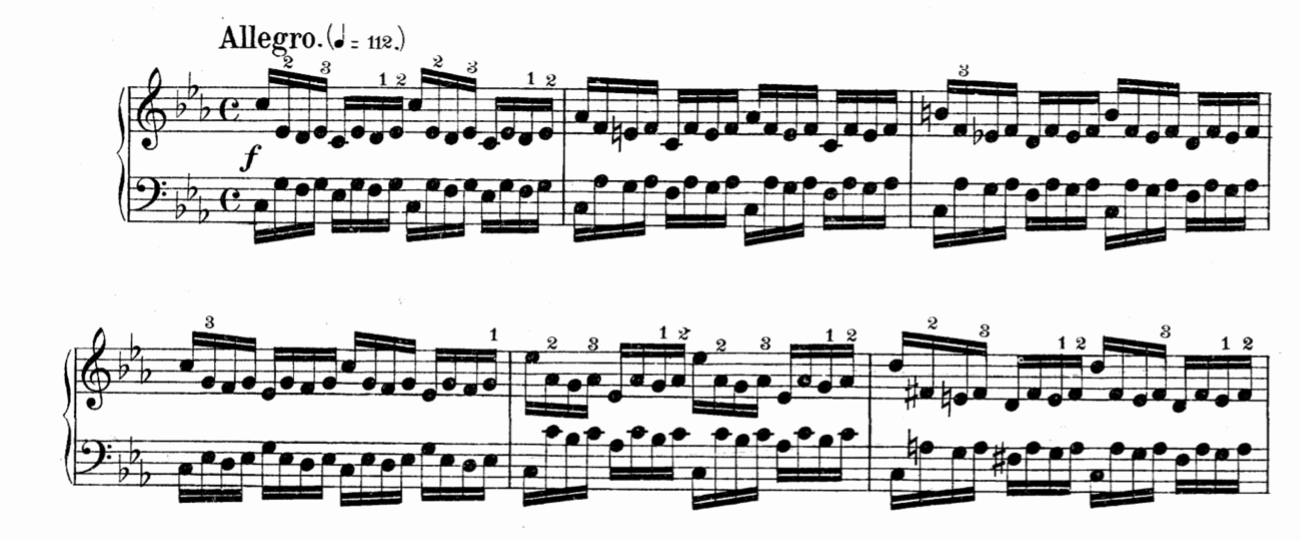
\includegraphics{figures/bach-first-motive.png}
%    \caption{The first of several motives found in the \textit{Prelude in C Minor %\cite{Bach_1722}}}
%    \label{fig:bach-first-motive}
%\end{figure}

A second motif is introduced in the coda [INSERT FIGURE OF CODA], which is marked by a change in both the piece's texture and tempo. An arpeggiated chord is followed by a rapid succession of thirty-second notes, as seen in figure [INSERT FIGURE OF SECOND MOTIF]. This new motif is repeated twice, after a succession of sixteenth notes ends the prelude on a Picardy third.[INSERT FOOTNOTE ABOUT PICARDY THIRD DESCRIPTION \& SOURCE]
%See figure %\ref{fig:bach-second-motive}.
%
%\begin{figure}
%    \centering
%    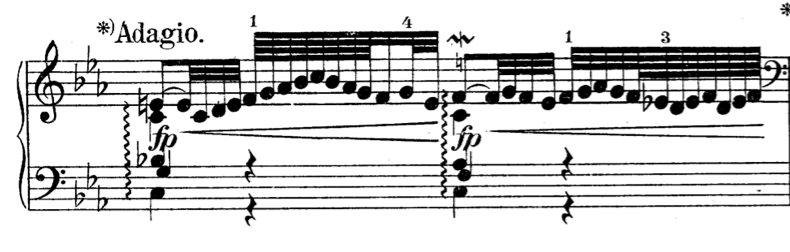
\includegraphics{figures/bach-second-motive.png}
%    \caption{The second motive, found in the \textit{ Prelude in C Minor} %\cite{Bach_1722}}
%    \label{fig:bach-second-motive}
%\end{figure}
%

The \textit{Fugue in C Minor} is an example of a fugue written in three voices. [INSERT FIGURE OF THREE VOICES CIRCLED AND UNDERLINED, WITH DESCRIPTIONS OF EACH] It is a balanced piece, with structure and interactions between the three voices, soprano, alto, and bass--or subject, and two countersubjects. Structurally, the fugue starts with an exposition [INSERT FIGURE OF EXPOSITION], which marks the introduction of the subject line in the alto voice [INSERT FIGURE OF SUBJECT], as in figure [FIGURE]. This subject then is seen in the soprano and bass voices [INSERT, AS SEEN HERE]
%%figure \ref{fig:bach-fugue-subject}. The subject then expands into the soprano %and bass voices. 
%
%\begin{figure}
%    \centering
%    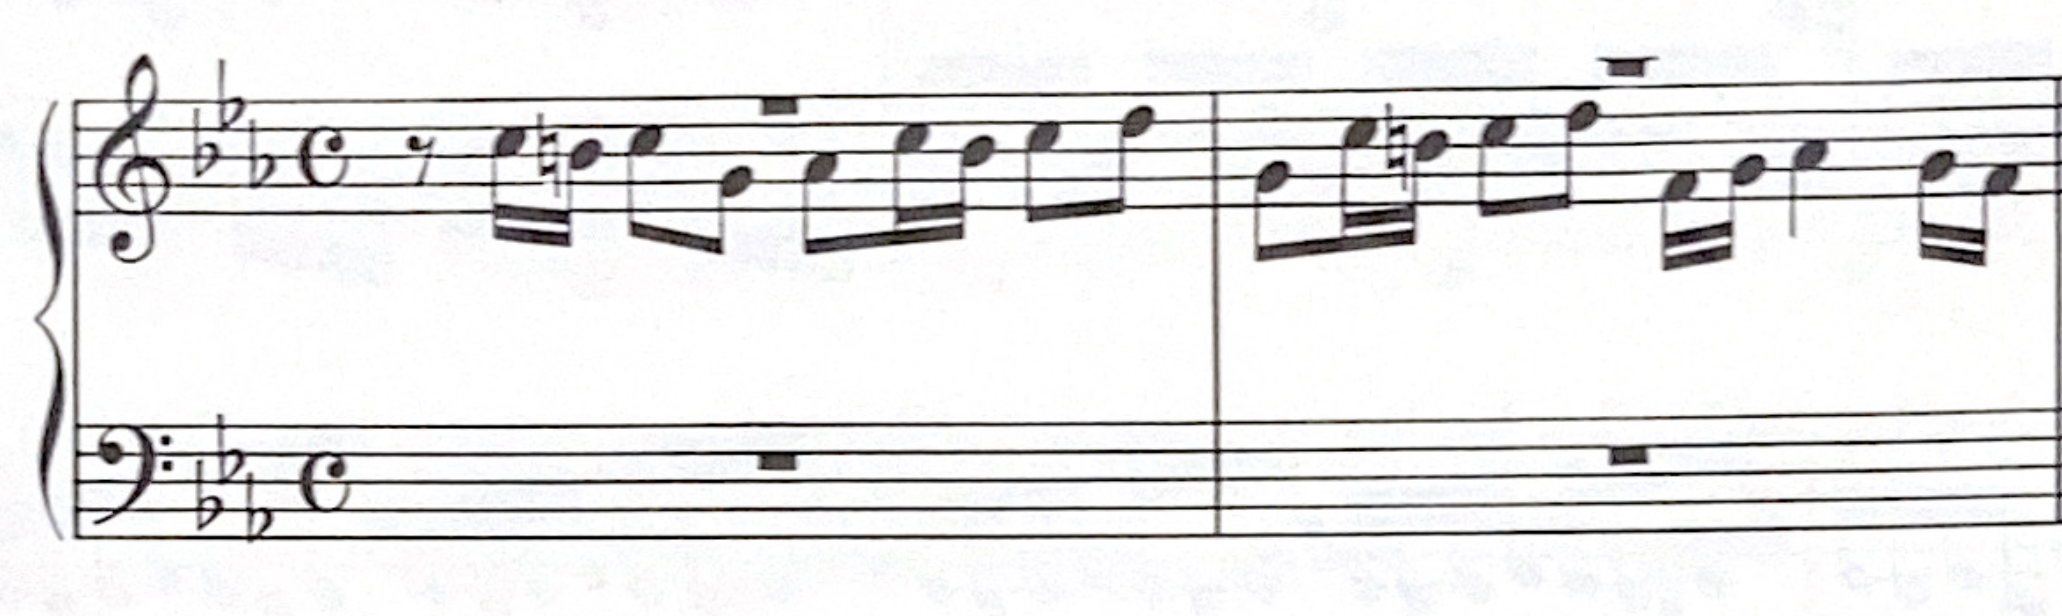
\includegraphics{figures/bach-fugue-subject.png}
%    \caption{The subject of the \textit{Fugue in C Minor} \cite{Bach_1722}}
%    \label{fig:bach-fugue-subject}
%\end{figure}

The piece's third measure introduces the first countersubject in the sorprano voice, as in figure [INSERT FIRST COUNTERSUBJECT]

%Bar three introduces the piece’s first countersubject in the soprano voice, as in %figure \ref{fig:bach-fugue-countersubject}.

It is an inversion [INSERT DEF OF INVERSION] of the subject's melodic line. The second countersubject is rhythmically indicated in the second half of the first countersubject before it is introduced on its own. [INSERT EXAMPLE OF RHYTHMIC INDICATION] The second countersubject first fully appears in measure seven, as in figure 

%figure %\ref{fig:bach-second-countersubject}\cite{Bach_1722}}.
%
%\begin{figure}
%    \centering
%    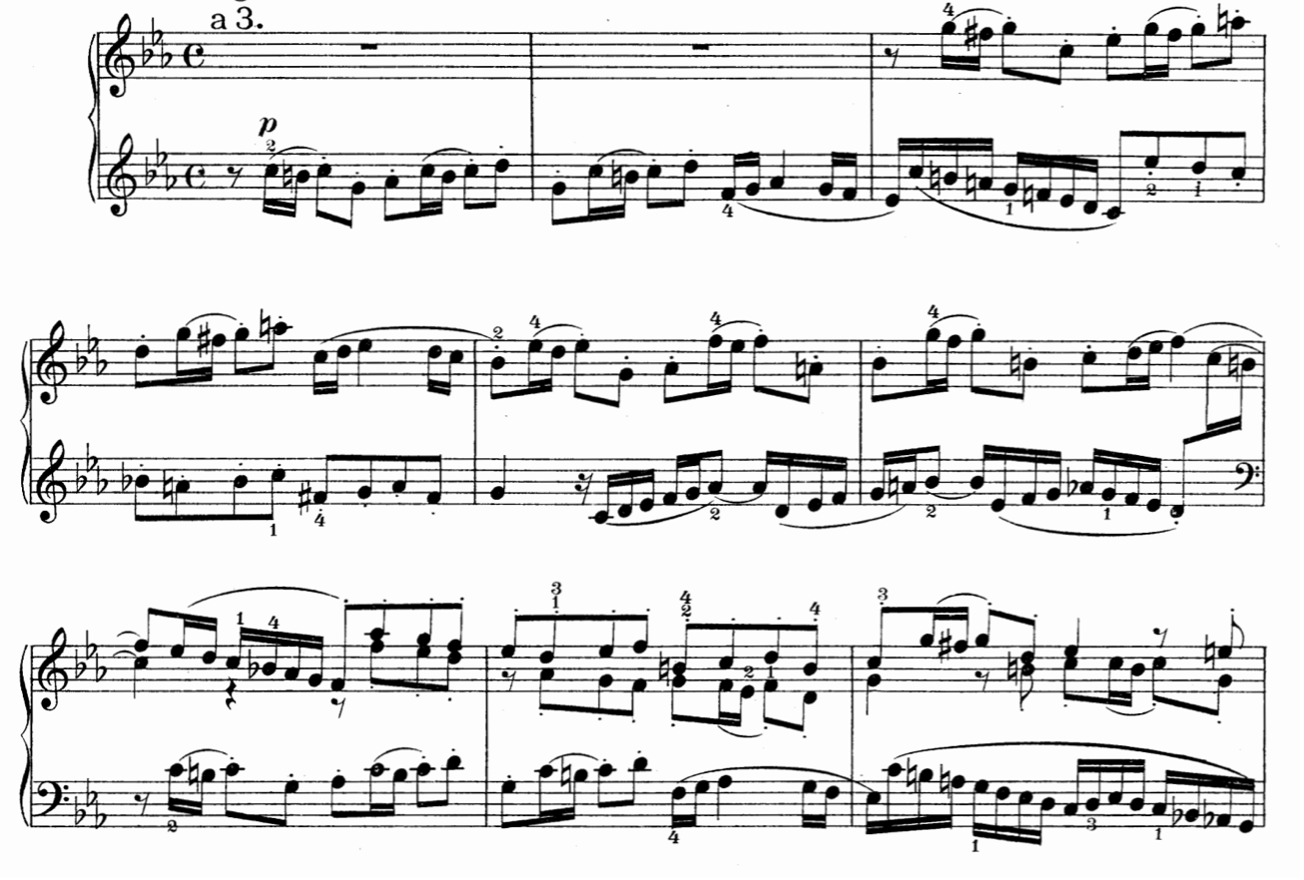
\includegraphics{figures/bach-fugue-countersubject.png}
%    \caption{The soprano raises the first countersubject in the \textit{Fugue in %C Minor} \cite{Bach_1722}}
%    \label{fig:bach-fugue-countersubject}
%\end{figure}
%
%\begin{figure}
%    \centering
%    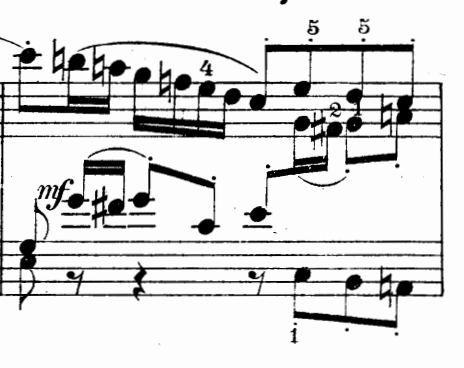
\includegraphics{figures/bach-second-countersubject.png}
%    \caption{The second countersubject found in the \textit{Fugue in C Minor}, in %full.}
%    \label{fig:bach-second-countersubject}
%\end{figure}
%

Harmonically, the \textit{Fugue in C Minor} has a strong emphasis on minor keys, for dramatic effect [INSERT EXAMPLE OF THIS HERE]. In the fugue's tension map\footnote{This is defined as a chart which details when there is tension in the music, and when the tension is resolved. Tension can be created through a chord's function, rhythm, or other methods.} there is more than a simple exposition\footnote{This is generally defined to be the section at the beginning of the piece, or near the beginning, in which one or more themes are presented according to a particular plan. These themes will be the basis of the rest of the movement or piece. In fugues specifically, the exposition is the opening section in which the voices enter one by one. Each voice states the principle theme (the subject), followed by the countersubject. All the voices after the fugue will wait to enter until the preceding voice has completed its statement of the subject. More information can be found in \citeauthor{Walker_2001_Exposition}, \citeyear{Walker_2001_Exposition}}, subject entries, and coda\footnote{This is defined as the last part of a piece or melody, in which there is an implication that there is some addition being made to a standard form. In a fugue, this then refers to anything occurring after the last complete entry of the subject has been heard. Read more in \citeauthor{Bullivant_2001}, \citeyear{Bullivant_2001}}. The sequence of subject entries in the development section is asymmetric, as seen in figure [INSERT EXAMPLE HERE]. There are three subject entries in the soprano and alto voices, two entries in the soprano voice, and one in the alto voice; the fourth voice is introduced in the soprano voice, instead of the bass voice.